\documentclass[border=3pt,tikz]{standalone}
% Shared look for every TikZ figure in these notes.
% Included by each standalone figure file; also keeps the figures consistent
% with the colours used in the PDF and on the website.

\usepackage{tikz}
\usepackage{pgfplots}
\pgfplotsset{compat=1.18}
\usetikzlibrary{arrows.meta, decorations.markings, decorations.pathmorphing,
                patterns, calc, positioning}
\usepackage{amsmath}

% Series colours are the three validated categorical slots also used by the
% interactive widgets, so a path drawn in the printed notes and the same path on
% the website are the same colour. They clear the colour-vision-deficiency and
% contrast checks as a set; every path is direct-labelled as well, so colour is
% never the only thing carrying identity.
\definecolor{duPurple}{HTML}{68246D}
\definecolor{duBlue}{HTML}{2A78D6}
\definecolor{duRed}{HTML}{EB6834}
\definecolor{duGreen}{HTML}{1BAF7A}
\definecolor{duGrey}{HTML}{6B6B6B}

\tikzset{
  axisline/.style   = {-{Stealth[length=3mm]}, line width=0.7pt, black},
  path1/.style      = {duBlue,   line width=1.1pt},
  path2/.style      = {duRed,    line width=1.1pt},
  path3/.style      = {duGreen,  line width=1.1pt},
  statedot/.style   = {circle, fill=black, inner sep=1.4pt},
  arrowhead/.style  = {decoration={markings,
                        mark=at position #1 with {\arrow{Stealth[length=2.6mm]}}},
                       postaction={decorate}},
  lbl/.style        = {font=\small},
  slbl/.style       = {font=\footnotesize, duGrey},
  workfill/.style   = {duPurple, opacity=0.16},
}

\begin{document}
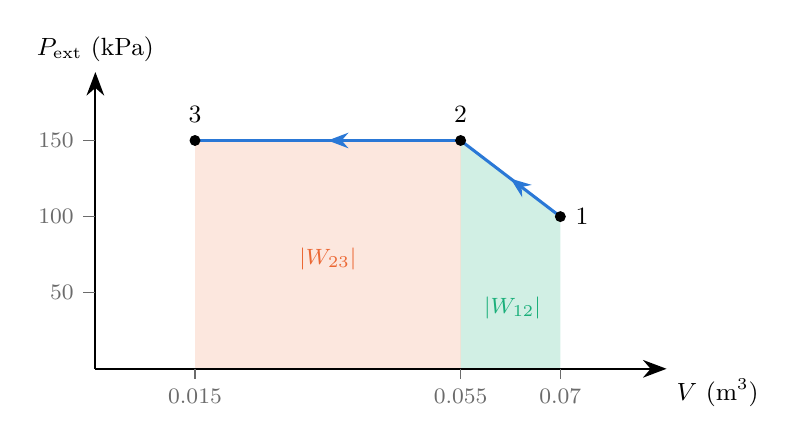
\begin{tikzpicture}[x=2400pt, y=0.55pt]
  % 1 -> 2 : trapezium ; 2 -> 3 : rectangle
  \fill[duGreen, opacity=0.20] (0.055,0) -- (0.055,150) -- (0.07,100) -- (0.07,0) -- cycle;
  \fill[duRed,   opacity=0.16] (0.015,0) rectangle (0.055,150);

  \draw[axisline] (0,0) -- (0.086,0) node[below right, lbl] {$V$ (m$^3$)};
  \draw[axisline] (0,0) -- (0,195) node[above, lbl] {$P_\text{ext}$ (kPa)};

  \draw[path1, arrowhead=0.5] (0.07,100) -- (0.055,150);
  \draw[path1, arrowhead=0.5] (0.055,150) -- (0.015,150);

  \node[statedot] at (0.07,100)  {}; \node[lbl, right=2pt] at (0.07,100) {1};
  \node[statedot] at (0.055,150) {}; \node[lbl, above=3pt] at (0.055,150) {2};
  \node[statedot] at (0.015,150) {}; \node[lbl, above=3pt] at (0.015,150) {3};

  \node[slbl, duGreen] at (0.0628,40) {$|W_{12}|$};
  \node[slbl, duRed]   at (0.035,72)  {$|W_{23}|$};

  \foreach \vv/\lab in {0.015/0.015, 0.055/0.055, 0.07/0.07} {
    \draw[duGrey, line width=0.4pt] (\vv,0) -- (\vv,-7);
    \node[slbl, below] at (\vv,-7) {\lab};
  }
  \foreach \yy in {50,100,150} {
    \draw[duGrey, line width=0.4pt] (0,\yy) -- (-0.0018,\yy);
    \node[slbl, left] at (-0.0018,\yy) {\yy};
  }
\end{tikzpicture}
\end{document}
